\documentclass{article}
\usepackage{pgf-umlcd}
\usepackage{fullpage}
\begin{document}
textwidh \the\textwidth
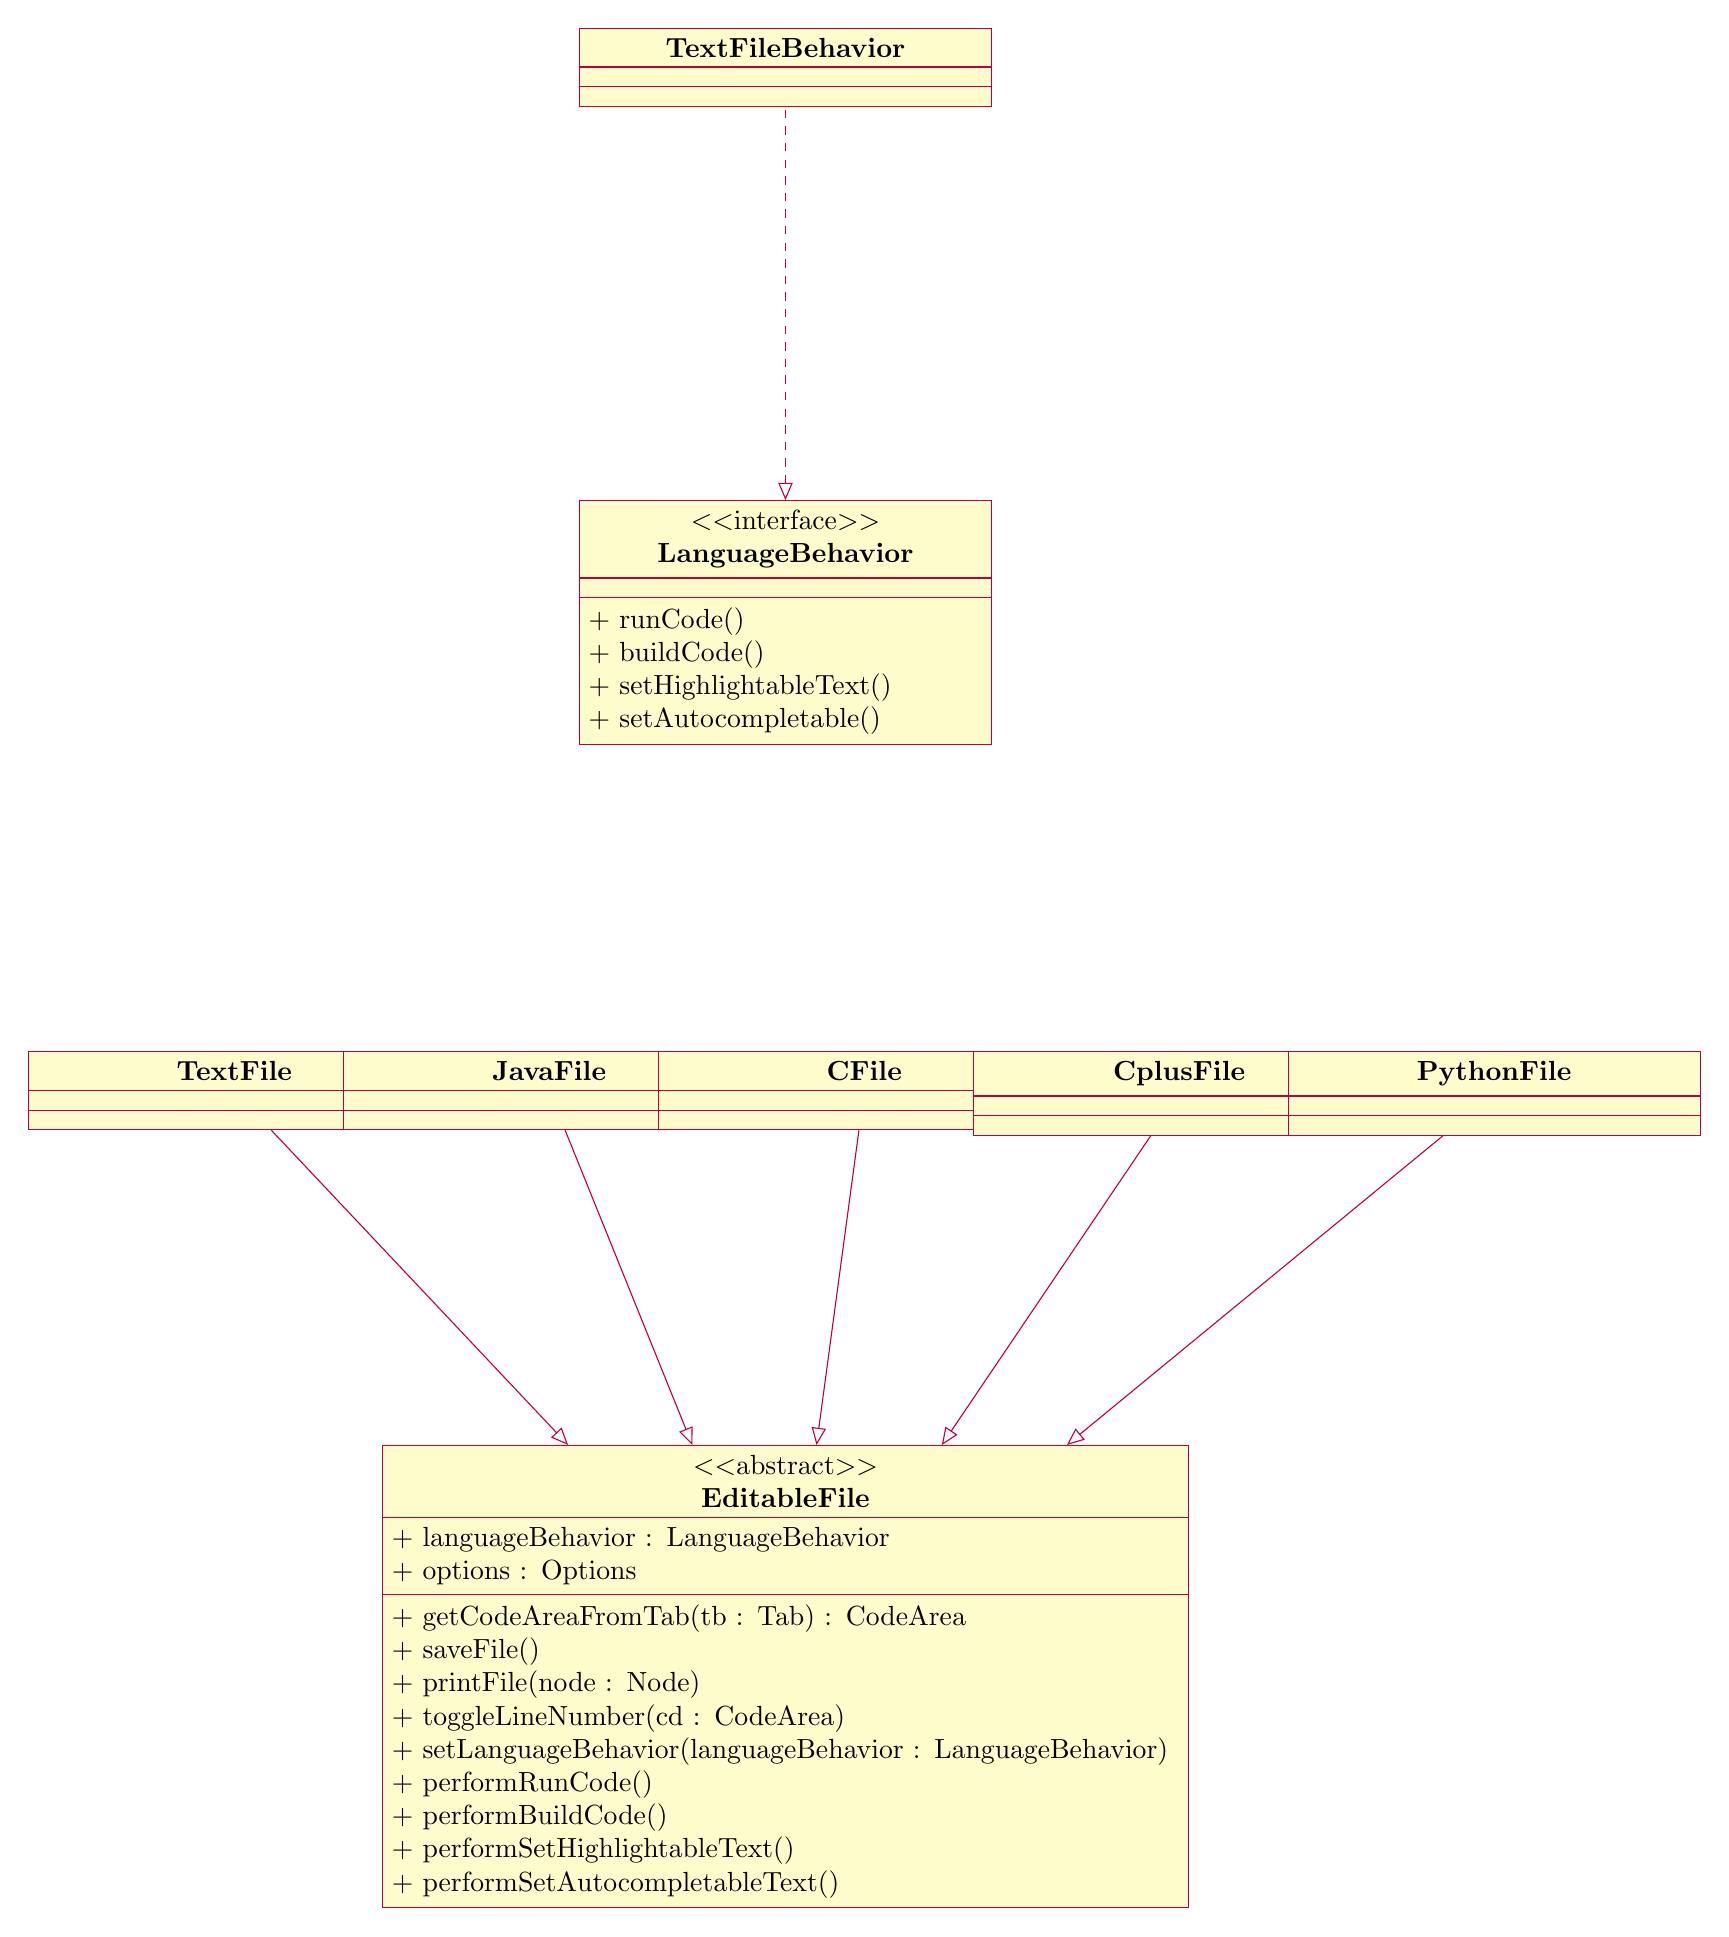
\begin{tikzpicture}

  \begin{abstractclass}[text width = 10cm]{EditableFile}{8,0}
    \attribute{+ languageBehavior : LanguageBehavior}
    \attribute{+ options : Options}
	\operation{+ getCodeAreaFromTab(tb : Tab) : CodeArea}
	\operation{+ saveFile()}
	\operation{+ printFile(node : Node)}
	\operation{+ toggleLineNumber(cd : CodeArea)}
	\operation{+ setLanguageBehavior(languageBehavior : LanguageBehavior)}
	\operation{+ performRunCode()}
	\operation{+ performBuildCode()}
	\operation{+ performSetHighlightableText()}
	\operation{+ performSetAutocompletableText()}
  \end{abstractclass}


  \begin{class}{TextFile}{1,5}
	\inherit{EditableFile}	
    \end{class}


  \begin{class}{JavaFile}{5,5}
	\inherit{EditableFile}	
    \end{class}

  \begin{class}{CFile}{9,5}
	\inherit{EditableFile}	
    \end{class}

  \begin{class}{CplusFile}{13,5}
	\inherit{EditableFile}	
    \end{class}

  \begin{class}{PythonFile}{17,5}
	\inherit{EditableFile}	
    \end{class}

  \begin{interface}{LanguageBehavior}{8,12}
    \operation{+ runCode()}
    \operation{+ buildCode()}
    \operation{+ setHighlightableText()}
    \operation{+ setAutocompletable()}
  \end{interface}

    \begin{class}{TextFileBehavior}{8,18}
      \implement{LanguageBehavior}
    \end{class}

\end{tikzpicture}
\end{document}
